\chapter*{General Discussion\markboth{General Discussion}{}}
\addcontentsline{toc}{part}{General Discussion}
The research reported in this thesis aimed at identifying daily practices of adult lifelong learners and how they can be supported with technology in and across contexts. Therefore in a first step everyday patterns of lifelong learners were identified and mapped on a context model. From the perspective of the content, best practices to access educational resources from mobile devices were pinpointed as well as potential approaches to bind digital educational resources to physical spaces. Based on these findings, in a second step a set of prototypes to support lifelong learners were designed constituting a substantial base of tools and knowledge towards its evaluation in experimental settings. In a third step, these tools are evolved with the aim to facilitate lifelong learners to manage everyday life and learning activities in a more enjoyable and efficient way.
\section*{Main findings}
This research has concluded in the following achievements that are formulated together with future research challenges for ubiquitous support of lifelong learners with technology:

\subsection*{Understanding how lifelong learners learn using technology}
The results from the survey in \textbf{Chapter 1} shed light on different patterns describing how lifelong learners use their mobile devices to learn. Portable computers are perceived as the most commonly used device to learn. Participants owning a smartphone reported to be more constantly motivated to learn throughout the day in contrast to feature-phone users (See figure \ref{survey_fig:2}), probably due to their perception of replacing �lost time� into perceived �productive time� when changing the context, commuting or in waiting times. Likewise, participants reported that they usually multitask while accomplishing learning activities with their mobile devices, especially \textit{listening} to content in which they reported to devote more time and in longer time slots. Regarding their preferred physical space to learn using mobile devices, there is an association between the learning activity being performed (i.e. \textit{reading, listening, writing, watching}) and the concrete location where it takes place (i.e. living room, kitchen, bathroom. See figure \ref{survey_fig:5}). Additionally, the reports from the participants in the survey indicate that learning experiences are disrupted, whereas �finding a suitable time slot to learn during the day� is perceived as the most frequently found barrier.  

The findings concluded in this chapter are based on the reports from 147 participants from very specific contexts (three Dutch and Spanish universities, two high schools from Belgium and The Netherlands, two companies, one academy for skills-training). The questionnaire has ben released\footnote{Tabuenca, B. (2012) A Questionnaire for Lifelong Learners on Mobile Usage Habits, DSpace, Open Universiteit in the Netherlands, NELLL. Heerlen. Available online at  http:// hdl.handle.net/1820/4296} under open access so these results con be contrasted with further communities, contexts and countries. In coming research, we suggest to survey larger populations in subsequent iterations so these results can be documented and mapped to the ongoing evolution of the technology.

The results from the longitudinal study reported in \textbf{Chapter 9} conclude in the following time-patterns describing how lifelong learners learn throughout the day and the week. On the one hand side, students were able to log their study-time on personal mobile devices along the day with three different levels of intensity with regard to the number of time-logs performed (see figure \ref{fig:sload_10}): 1)  High Intensity. Time ranges between 9h to 15h and 18h to 22h. 2) Medium Intensity. Time ranges between 8h to 9h, 15h to 18h and 22h to 0h. 3) Low Intensity. Time ranges between 0h and 8h. On the other hand, findings show average time-logs per day fluctuate between 58 minutes to 83 minutes along the week (See table \ref{tbl:studyload_table5}). Students reported more minutes and more time-logs on Thursdays and Sunday. Longer time-logs were reported on Tuesdays and Wednesdays whereas the shorter ones are reported Mondays and Fridays.

Lifelong learners explored how they do learn logging, tracking and monitoring one of the dimensions of context \citep{Specht2009}: \textit{time}. In further research, this tool represents a suitable approach for lifelong learners to track their learning habits while observing at the rest of the dimensions in their context (figure \ref{Esm_fig2}), namely, \textit{location} (i.e. where do I learn?), \textit{relation} (i.e. who with do I learn?), \em environment \em (i.e. which environmental circumstances affect me while learning?) and \em artefact identifier \em (i.e. which artefacts do I use to learn?).

\begin{figure}
     \centering
     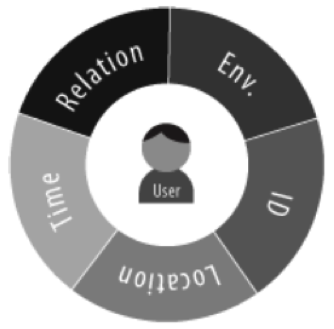
\includegraphics[width=0.4\linewidth]{img/Esm_fig2}
     \caption{Dimensions of mobile context \citep{Specht2009}}
     \label{Esm_fig2}
\end{figure}

\subsection*{Facilitate ubiquitous access to digital learning resources}
\textbf{Chapter 2} reviews the state-of-art of learning repositories featuring mobile access to digital resources. This review has concluded identifying different implementations to access content indexed by GPS coordinates, compass orientation, gesture recognition via accelerometer, radio frequency identification, infrared, visual code scanning, Bluetooth approximation, text-marker recognition or image recognition. Looking at the granularity of the resources, we found that easy to create and to consume contents on mobile devices, are those whose unit of construction is text, audio or video (minimum granularity). Going in depth to technical implementations, the conclusions of the review pinpoint to server architectures based on RESTful web-services featuring an Application Programming Interface (API), as well as HTML5 client, as suitable software implementations to facilitate content accessibility and scalability.  

Videos represent a big proportion of the learning materials provided in online courses for mobile access. Most of the times, these videos are released in a LMS or shared in public repositories (i.e. YouTube, Vimeo). Watching a video requires the user to switch-on the device (x minutes), open a browser, login the platform, navigate to look for the desired resource (y clicks), and finally display the video on the mobile device (low resolution). This approach presents time, interaction and qs. In \textbf{Chapter 3}, we pilot the NFC-MediaPlayer, an ecology of resources comprising NFC tags, a multimedia casting tool, and a learning content referratory to cast videos from a mobile device to an HDMI display interpreting the commands (i.e. play, pause, forward, cast) of the NFC tag that is tapped with the mobile device. This novel ecology facilitates seamless access to video contents reducing the time to start the learning activity, reducing the number of clicks to access the learning content (to zero clicks), and casting in High-Definition quality, learning contents that are normally casted in small-sized screens on mobiles, tablets or laptops. Additionally, we share the �know how� releasing the source code under open license to foster its scalability fur further applications and communities.

% Findings reported in \textbf{Chapter 2} show different channels to enable ubiquitous access to digital learning resources stored in content repositories using mobile devices. The scalability of new mobile clients providing access to content stored in repositories is highly dependant on the existence of an API, as well as the granularity of the content which is served. Hence, we conclude that learning contents offered with a low granularity (i.e. text, video, audio) and repositories implementing RESTFul web-services facilitate access to digital resources to mobile app developers, smartphone users and consequently to a broader range of lifelong learners.

\subsection*{Linking learning activities with everyday life activities and the physical world objects}
\textbf{Chapter 2} identified NFC technology as a prominent trend in the field of mobile technology in the last years. This technology is particularly relevant for lifelong learners due to its reduced complexity to accomplish predefined actions (zero-clicks) and facilitating a smooth integration of learning activities into physical spaces. \textbf{Chapter 3} reviewed scientific literature in which NFC has been used with learning purposes and potential uses for learners are classified. As a consequence of this review,  \em activity recognition \em and  \em life logging \em are highlighted as relevant fields to link learning activities with everyday life activities. Indeed, lifelong learners' activities are scattered along the day and in different locations making it difficult to manage learning goals and to have an account of how much time is devoted to each one of them. Nevertheless, the results reported in \textbf{Chapter 1} show that lifelong learners frequently recur to preferred learning environments throughout their learning journey (physical spaces, devices, or moments). Sometimes the physical environment itself may relate to learning activities in other cases only temporal patterns might be of relevance while the physical location is not crucial. 

This research has provided cues for lifelong learners to introspect their autobiography as learners, to identify successful learning environments, to bind them to self-defined learning goals, to keep track of the time devoted to each goal, to monitor their progress, and consequently to understand how does he/she learn. The NFC-LearnTracker presented in \textbf{Chapter 6} supports lifelong learners in those functions, providing a suitable tool to foster awareness on preferred learning environments, to manage learning goals, to have an accurate account on time devoted to learn, and to analyze personal learning patterns.

The NFC-LearnTracker (released under open source), and the empirical studies identified in \textbf{Chapter 3} imply an important base of knowledge to scaffold potential scenarios linking learning activities with everyday life objects using NFC technology.  \cite{Livingstone2007} analysis on work-time and learning activities stresses the lack of longitudinal studies in job-related informal learning. In further research, the NFC-LearnTracker and its support to learning processes should be evaluated in real scenarios in which learners use their own NFC-enabled smartphones in longitudinal studies. This tool might be useful to determine whether there is a positive or negative correlation between learning performance and the duration of the learning moments, the time of the day, the location or the type of device used.

\subsection*{Awareness of available resources in everyday life}
This thesis has shown different cues to foster awareness on available resources, locations and moments to learn in everyday life using technology. In \textbf{Chapter 4} we proposed sampling of learning experiences on mobile devices as key benchmarks for lifelong learners to become aware on which learning task suits in which context, to set realistic goals, and to set aside time to learn on a regular basis. A classification framework for sampling of experiences on mobile devices has been presented as an approach to explore variations to deliver, dispatch, and answer notifications in context. This framework is not only useful when prompting notifications to second persons (e.g. from teacher to student), they are significantly more powerful and accurate when they are self-reports due to the fact that the lifelong learner has an intrinsic motivation to know himself as a learner and consequently to provide truthful reports having only himself as a reference. This classification framework is instantiated along the thesis for the prototypes presented in \textbf{Chapters 4, 6, 8 and 9}.

This self-reporting technique represents an interesting approach for lifelong learners to get actively involved in knowing their own learning day. The ESM instantiated in personal mobile devices is suited for lifelong learners to explore their own specific context, learning style, and available resources to model each learning moment.

\subsection*{Develop artefacts to support lifelong learners}
This thesis has resulted in the development of different artefacts and software prototypes that facilitate the implementation of educational designs as well as support the connection of informal learning experiences with formal learning activities in and across contexts. This research comprises the development of six different software tools shared in open source, namely, NFC-MediaPlayer (\textbf{Chapter 3}), ESM app (\textbf{Chapter 4}), Mobile Authoring Tool for ARLearn (\textbf{Chapter 5}), NFC-LearnTracker (\textbf{Chapter 6}), ecology of resources for effective time management (\textbf{Chapter 7}), and the LearnTracker framework (\textbf{Chapter 9}). 

The set of tools presented in this research facilitate connecting informal and formal learning experiences featuring author of learning resources in authentic scenarios, tracking and monitoring time devoted to learn across contexts, and providing seamless access to learning resources in frequently used lifelong learning scenarios. All these tools are released under open source\footnote{Source code repository of tools piloted in this thesis:\\ https://code.google.com/p/lifelong-learning-hub/source/clones} and might be adapted or extended in further research.

\subsection*{Identify barriers for digital competence in lifelong learners}
This thesis has demonstrated that the combined use of multiple devices might lead to important differences in digital competence from one learner to another. Findings from \textbf{Chapter 8} pinpoint to differences with regard to \textit{familiarity with the mobile device}, \textit{familiarity with the operating system of the device} and \textit{the complexity of the user interface} as key aspects to take into account when designing technology to support lifelong learners. Likewise, the results obtained in \textbf{Chapter 9} show that the \textit{usability of the tool}, the \textit{number of clicks} to accomplish an action, and the \textit{response time}, are key aspects to take into account in the design of tools to support lifelong leaners in long term.

\subsection*{Foster reflective practice on meta-learning}
All along this thesis we have explored the effectiveness of mobile notifications to foster reflection on meta-learning. In a first step (\textbf{Chapter 4}) we explored the variables affecting the user when sampling experiences on mobile devices and the ESM app was developed to identify user preferences with regard to the way to receive, dispatch and answer notifications on mobile devices. The results of the pilot evaluation show that learners preferred to receive notifications \textit{on-demand} rather than \textit{time-scheduled} or \textit{random basis}.  Additionally, they preferred prompt notifications as well as answer notifications in \textit{text} format, in contrast to \textit{audio}, \textit{picture} or \textit{audio} formats.

In the two studies presented in \textbf{Chapter 8}, we used reflection amplifiers \citep{Verpoorten2012} instantiated with mobile notifications to make what users learn, a deliberate object of attention. Findings in the first experiment show that (secondary school) students do not have a habit to see themselves as learners and to develop a professional awareness about their daily activity at work/school. In the second experiment we researched variations in the �timing�, �frequency�, and �complexity� of notifications fostering reflective practice on learning, and its impact on �knowledge� and �motivation�. Findings in this experiment show better �knowledge� scores for the group of learners that were assigned with the least complex interactions on mobile devices during the reflection exercise. 

Based on the lessons learned from these experiences, the longitudinal study described in \textbf{Chapter 9} evolved the NFC-LearnTracker presented in \textbf{Chapter 6}, to observe variations in the �timing� and �content� of the notifications. Findings reveal positive effects of tracking learning time in �time-management� skills. These results not only provide evidence of the benefits of recording learning time, but also suggest relevant cues on how mobile notifications should be designed and prompted towards self-regulated learning.

\subsection*{Self-defined internal feedback}
The differentiation among external and internal feedback is crucial if one investigates the effects of feedback as a self-regulated learning process \citep{Narciss2007}. Hence, the last phase of the research shifts the perspective from externally designed notifications (i.e. designed by the teacher, instructional designer or researcher) to self-designed notifications (i.e.designed by the learner) evolving the NFC-LearnTracker to an ecology of resources in which lifelong learners can design notifications served via an ambient learning display \citep{Borner2013}, and map them to events happening along the learning process. This ecology lets the user configure which signal fits better each one of these events (see Table \ref{tbl:nfceco_table1}).

In further research this tool might support to investigate the impact in self-regulated learning of externally designed notifications (external feedback) in contrast to self-defined notifications (internal feedback).

\section*{Limitations of this research}
By identifying daily practices from lifelong learners this thesis has contributed towards a common understanding of how lifelong learners learn to support them with ubiquitous technology. However, several factors limited the conducted research:

Regarding \textit{understanding how lifelong learners learn using technology} , the results reported in \textbf{Chapter 1} are based on personal perceptions. Concepts like \textit{motivation to learn} or \textit{learning intensity} might be understood differently depending on the user that is answering the questionnaire. Additionally, the time patterns found in \textbf{Chapter 9} might be influenced by the assignments scheduled by the teachers for this specific course. There is a need to extend this research to larger groups from several disciplines to obtain a more accurate vision on how lifelong learners learn (throughout the day and along the week) independently on the courses they are enrolled.

Regarding \textit{facilitating ubiquitous access to digital learning resources} , the results presented in \textbf{Chapter 2} and \textbf{Chapter 3} show different shortcuts facilitating access to content stored in repositories. Nevertheless, most of the technologies presented in these reviews were piloted in special settings (i.e. lab experiments, restricted scenarios, augmented reality) that might not be extrapolated to real case scenarios. 

Regarding \textit{linking learning activities with everyday life activities and the physical world objects} , the evaluation of the NFC-LearnTracker has been performed in an artificial context (technology enhanced learning workshop). This tool should be tested in longitudinal studies with personal mobile devices and in lifelong learning settings. In a realistic scenario, the single decision to start using the tool should be triggered by an intrinsic motivation from the user to explore own learning patterns rather than an externally imposed tool. 

Regarding \textit{awareness of available resources in everyday life} , the pilot presented in \textbf{Chapter 4} has raised the following limitations: first, this pilot was tested in an exceptional learning context. Real lifelong learning scenarios imply daily routines like workplaces, transitions, etc.; second, the duration of the experiment was too short. Modelling one�s lifelong learning day implies a long-term experiment in which moments of the day and moments of the week are explored. 

Regarding the \textit{development of artefacts to support lifelong learners} , we have released several prototypes that might need adaptations depending on the contingencies of the context in which they are evaluated, and the version of the operating system in which they are deployed. Most of the artefacts presented in this thesis were developed for Android devices. These tools might need to be extended to further operating systems in future developments.

Regarding \textit{foster reflective practice on meta-learning} , the experiment presented in \textbf{Chapter 4} involved 12 voluntary researchers in the field of Technology Enhanced Learning (TEL). The small-scale of the participation, the short duration of the experiment, and the fact the participants had an expertise in TEL might have biased the reported results. These results should be contrasted with further larger studies.

Most of the conclusions reported in \textbf{Chapter 9} are based on the recordings from 13 students taking part in an online university course during 4 months. Findings reported in this thesis might need to be contrasted with larger groups. Some of the effects identified in the intermediate measures might be moderated as a consequence of sequencing effects, and not only caused by the treatment delivered during that specific treatment. More research is needed providing these treatments to independent groups.

Lifelong learners model daily learning routines based on intrinsic motivations and personal decisions taken in real circumstances. The tools used in these studies were not discovered by the learners themselves, but rather offered to them from external researchers. Thus, initiatives to mentally evoke what they have learned throughout the day to turn the learning experience into a deliberate object of attention and reflection are more powerful when they come from personal motivations rather than from external invitations.

Most of the work reviewed in this thesis is limited to scientific literature. Nevertheless, a big proportion of lifelong learners' practices are not documented because they are implemented based on personal understandings and consequently do not have a relevant scientific value. In future research, interviews might help to understand further patterns on how lifelong learners learn by collecting hedonic and qualitative data of best practices from an individual perspectives. 
